%% =====================================================================
\section{相关工作}
\label{sec:related_work}
%% =====================================================================

%% 相关工作按问题类型回顾,不作「四层定位」。旧文献以引文簇保留,叙述以近作为主。

动态调度的一个基本问题是：扰动发生后，重调度范围划在什么对象上，即改哪些、其余保持不动。
已有文献把这一范围划在不同对象上——工序或时间轴、排他资源上的占用先后、
受影响的车辆，以及带运输的柔性作业车间中的工序集合。
下面按这四类回顾各自做了什么、尚未覆盖什么，并在表~\ref{tab:position} 中做汇总。

\subsection{作业车间的局部重调度}
\label{sec:rw_aor}

对机器故障、插单等工序事件，按受影响工序划定重调度范围，在带 AGV 的动态调度中仍被采用。
Zhang 等~\cite{zhang2023energy} 处理机器故障与插单，恢复范围取故障后尚未加工的工序；
Tang 等~\cite{tang2026dynamic} 按扰动影响把工序与配送任务分为保留、继续、重构，
并把完全重调度、部分重调度与右移并列，指出右移保住稳定性、让出优化空间。
本节与下节据以定位的转述，所本原句一并列于表~\ref{tab:refcheck}。
这一做法可上溯至受影响工序重调度(AOR)~\cite{abumaizar1997rescheduling,subramaniam2003maor}：
只重排被扰动直接或间接波及的工序。
沿时间轴划界与失败后扩大范围同样已有文献研究过，包括 match-up~\cite{akturk1999matchup}
与增量扩大时间窗的 Local Rescheduling~\cite{kuster2007local}。
右移则不判定谁受影响，把未完成部分整体后推。
滚动时域与分解式方法在规模与质量之间折中~\cite{zeitrag2025novel,zhao2019decomposition}；
综述见~\cite{vieira2003rescheduling,ouelhadj2009survey}。

这些工作表明，划定范围再局部重调度并不是新问题，前提是扰动首先作用在工序上。
一旦扰动只使走廊不可通行而不改指派，按该方法划出的范围可以为空，原排程却已不可行。

\subsection{排他资源上的占用先后}
\label{sec:rw_ag}

「谁先占用同一排他资源」被建成图，在铁路调度中已有系统研究。
Mascis 与 Pacciarelli~\cite{mascis2002alternative} 的 alternative graph
把析取图推广为：顶点是作业对闭塞区段的占用，固定弧表示路径先后，
成对的 alternative arc 表示谁先通过该区段。
D'Ariano 等人~\cite{dariano2007branch} 用该模型做列车实时重调度，
扰动后重算无冲突时刻表，并尽量接近原计划。
同走廊上的让行关系与 alternative arc 表达的是同一类先后。

与本文不同的是用法。对每一处争用，alternative graph 给出两条互斥的弧
（甲先通过，或乙先通过），排程就是从中选定一条：
选定后图中不能出现正权回路，时刻表才可行，并尽量使目标最优——占用先后因此是决策变量。
本文的计划已经排好，谁先通过哪条走廊已经确定，不再选择先后，
只按这些既定的让行与接续关系，把扰动后必须作废的原走廊占用纳入重调度范围。
此外，铁路模型把闭塞区段当作机器，工序与占用在同一张图上，
区段不可用即为工序事件，因此不存在「范围划在工序依赖图上而遗漏走廊阻断」的问题。
柔性作业车间中加工与走廊占用是两套对象，现有的 AOR 划界并不利用占用先后关系。

\subsection{无冲突多车路径的局部重规划}
\label{sec:rw_mapf}

在多智能体路径规划中，只为受影响者进行重调度、其余视为动态障碍，已是标准做法。
Švancara 等人~\cite{svancara2019online} 在在线 MAPF 中给出
% selfcheck:allow-term 「受影响集合」此处指 MAPF 独立性检测的输出,不是本文机制的名字
Replan All、Replan Single 与 Replan Affected，并用在线独立性检测确定受影响集合；
Malka 等人~\cite{malka2024online} 在地图不准确时，同样只为受观测变化影响的车辆重规划。
% selfcheck:allow-term 「时空占用」是 MAPF 的既有术语,此处在转述该文献,不指本文的走廊占用
无冲突路径规划把时空占用作为一等约束，但起终点通常由外部给定~\cite{zhang2024guidance}。

上述做法已经把「只改受影响者、其余保持原计划」做成标准机制，本文沿用这一机制。
与本文设定的不同在于：这类工作只有车辆的起终点，没有工件—工序—机器指派，
因而不会出现「重调度范围按工序依赖图划定、走廊阻断因找不到受影响工序而被遗漏」的情形。
% selfcheck:allow-term 「受影响集合」此处是两法共用的中性说法,后半句即在说它是检测算法的输出
就受影响集合如何得到而言，MAPF 用独立性检测找出受影响车辆，得到的是检测算法的输出，随实现方式和停止条件而变。
本文给出的预约影响集则不同：依赖边一经给定，一条占用是否属于该集，
只取决于它能否从起点沿这些边到达，与随后用哪一种改路算法无关
（第~\ref{sec:containment}~节）。

\subsection{考虑运输的柔性作业车间调度}
\label{sec:rw_position}

考虑运输车辆的柔性作业车间调度已有系统综述~\cite{xin2025review}。
近期组合优化工作仍普遍把行驶时间取为按位置对索引的常数矩阵，
并在此之上发展约束规划、元启发式与知识引导搜索~\cite{meng2025cp,qin2026knowledge,fu2025integrated}。
该约定下车辆并不争用同一路段，走廊阻断在模型里没有对应对象，无法被检验。

一旦用时间窗记录走廊占用，加工先后与走廊占用同时进入模型。
拥堵感知派车可用局部密度等代理量选车，而不改机器指派~\cite{kim2026congestion}。
把柔性指派与无冲突运输联合建模的工作相对较少：
van Os 与 Basten~\cite{vanos2026exact} 形式化了带无冲突运输约束的柔性作业车间调度，
并以分解方法在多数基准算例上取得可证最优，少数因限时未能保证最优性；
两阶段方案先固定排产再消解车辆冲突~\cite{sun2023integrated}；
亦有学习层排产、路径层消冲突、并以有限反馈连接的框架~\cite{li2026framework}。
但这些工作回答的是开工前如何排出可行且质量好的无冲突排程。

在本节所引工作中，走廊预约表与执行期扰动响应未同时出现：含预约表的工作排除了执行期故障，
处理执行期扰动的工作则没有预约表。
例如（原句见表~\ref{tab:refcheck}）：
Zhang 等~\cite{zhang2023energy} 在建模假设中写明忽略 AGV 之间的碰撞；
Sun 等~\cite{sun2023integrated}
用时间窗 Dijkstra 消解车辆冲突，却在假设中写明不考虑车辆的充电与故障、车辆始终可用，
并把设备维护与故障列为后续研究。

因此，缺口来自两个条件未同时具备：
工序级划界之所以成立，往往因为模型中没有走廊预约；含预约表的设定又排除了执行期扰动。
两者同时出现时，可直接沿用的只有按受影响工序划界的做法，
而它对不改变工序指派的走廊阻断给出空范围（第~\ref{sec:e1}~节实测 \PassMiss）。
本文处理的正是这一情形。

\begin{table}[t]
\centering
\caption{本文据以划出缺口的五处转述及被引原文（照录英文原句）。}
\label{tab:refcheck}
\footnotesize
\begin{tabular}{@{}p{0.23\linewidth}p{0.55\linewidth}p{0.14\linewidth}@{}}
\toprule
\textbf{本文的转述} & \textbf{被引原文} & \textbf{原文位置} \\
\midrule
Zhang 等~\cite{zhang2023energy} 的恢复范围取故障后尚未加工的工序 &
\emph{``Rearrange the unprocessed operations of current scheme considering the limit of
machine breakdown''} &
重调度流程 \\
\addlinespace
Zhang 等~\cite{zhang2023energy} 在建模假设中写明忽略 AGV 之间的碰撞 &
\emph{``The collision of AGVs are ignored.''} &
建模假设第 (7) 条 \\
\addlinespace
Tang 等~\cite{tang2026dynamic} 按扰动影响把工序与配送任务分为保留、继续、重构 &
\emph{``an event-driven partial rescheduling strategy is proposed, in which the disrupted
operations and delivery tasks are classified into three categories: retained, continued,
and reconstructed''} &
摘要 \\
\addlinespace
van Os 与 Basten~\cite{vanos2026exact} 在多数基准算例上取得可证最优，
少数因限时未能保证最优性 &
\emph{``For most benchmark instances, our LBBD-based approach finds optimal makespan
values. Because of time boxing, only in a few cases, the optimality of the found solution
cannot be guaranteed.''} &
摘要 \\
\addlinespace
Sun 等~\cite{sun2023integrated} 假定车辆始终可用、不考虑故障与充电，
并把设备维护与故障列为后续研究 &
\emph{``It does not consider the charging problem and fault problem of the AGVs, and AGVs
are always available''}；\emph{``Breakdowns and charging problems are not taken into
account.''}；\emph{``Future research will investigate the impact of equipment maintenance
and breakdowns on production scheduling''} &
假设列表、后续工作 \\
\bottomrule
\end{tabular}
\end{table}

\subsection{本文定位}
\label{sec:rw_claim}

\begin{table*}[t]
\centering
\caption{相关工作按\emph{划界对象}分类：每类工作把扰动后「需要改写什么」定义在哪种对象上。
「边界划在」为重调度范围所依附的对象；「有工序依赖图?」兼答该图是否与占用同图；
末行加粗者为本文所处的类别。}
\label{tab:position}
\small
\begin{tabular}{@{}p{0.16\linewidth}p{0.22\linewidth}p{0.14\linewidth}p{0.14\linewidth}p{0.24\linewidth}@{}}
\toprule
\textbf{类别} & \textbf{代表工作} & \textbf{边界划在} & \textbf{有工序依赖图?} & \textbf{与本文的关系} \\
\midrule
作业车间局部重调度 &
AOR~\cite{abumaizar1997rescheduling,subramaniam2003maor};
match-up~\cite{akturk1999matchup};
LRS~\cite{kuster2007local}；
带 AGV 的动态调度~\cite{zhang2023energy,tang2026dynamic} &
工序 / 时间窗 & 有 &
后文对照复现按工序划界与右移 \\
\addlinespace[2pt]
排他资源占用先后 &
alternative graph~\cite{mascis2002alternative}；
铁路实时重调度~\cite{dariano2007branch} &
闭塞区段占用 & 有，与占用在同一张图 &
让行关系同类；铁路用它选择车辆的先后，本文用既定先后划定需要改写的占用 \\
\addlinespace[2pt]
无冲突多车路径 &
Online MAPF~\cite{svancara2019online,malka2024online};
LMAPF~\cite{zhang2024guidance} &
受影响车辆 & 无 &
集内改路、集外保持已是标准做法 \\
\addlinespace[2pt]
带运输的柔性作业车间 &
常数矩阵~\cite{xin2025review,meng2025cp,qin2026knowledge,fu2025integrated}；
一体化排程~\cite{vanos2026exact,sun2023integrated,li2026framework} &
工序集合 & 有；预约表与执行期扰动未同时出现 &
\textbf{本文的位置} \\
\bottomrule
\end{tabular}
\end{table*}

综上，在考虑 AGV 无冲突路由的柔性作业车间中，排程同时用工序依赖刻画加工先后，
又用时间窗记录走廊占用。此时会出现前节所指缺口对应的情形：
走廊阻断等扰动并不使工序无法执行，原指派仍然有效，
但与受扰时段重叠的走廊占用已经失效，原排程不可行。
后文按工序依赖图划界的对照，复现的是第~\ref{sec:rw_aor}~节的做法。
本文主张把重调度范围改到走廊占用及其让行、接续关系上，得到由这些关系唯一确定的预约影响集。

%% =====================================================================
\section{走廊预约设定与执行期恢复问题}
\label{sec:problem}
%% =====================================================================

\subsection{系统设定与记号}
\label{sec:system_brief}

问题设定沿用带无冲突运输约束的柔性作业车间~\cite{vanos2026exact}。
本节一次写清后文用到的对象。一份可行排程 \(\mathcal{S}^0\) 视为给定输入：
它在 \(t=0\) 如何被搜索出来，不影响后文如何划定须改写的占用。

\subsubsection{车间与四组决策}
\label{sec:shop}

车间路由图 \(G=(V,E)\) 强连通。每台机器 \(m\) 由位于固定节点 \(\mathrm{loc}(m)\) 的机械臂执行加工，
下文的机械臂故障即指该机器失效；
\(v_0\in V\) 为装卸站。\(n\) 个工件、机器集合 \(M\)、同构单载车队
\(K=\{1,\ldots,N_A\}\)。工件 \(j\) 有固定工序链 \(O_{j1}\to\cdots\to O_{jn_j}\)；
工序 \(O_{ji}\) 的候选机器集为 \(\Omega_{ji}\subseteq M\)，在机器 \(m\) 上耗时
\(t^P_{jim}\)。一份完整排程同时确定四组决策：
(i)~每道工序的机器指派 \(x\);
(ii)~各机器上的工序加工顺序 \(\pi\);
(iii)~各次搬运的车辆指派 \(y\);
(iv)~每次车辆移动在 \(G\) 上的无冲突路径。
记
\[
\mathcal{S}=(x,\,\pi,\,y,\,R),
\]
其中预约表 \(R\) 是第 (iv) 组的显式记录，定义见下。

运输任务由指派\emph{派生}，不是输入：仅当相邻两道工序不在同一节点时才产生一次搬运。
一次搬运拆成两段——空载取货与满载送达——各段有自己的任务标签 \(u\)
（例如 \(O_{ji}\) 的空载段与满载段是两条记录）。装卸时间取为零：满载段在空载段抵达与工件就绪
二者中较晚的时刻起行，而送达时刻同时就是机器可开工、车辆可接新任务的时刻。
后文允许改写哪些占用、哪些占用保持原计划，以及如何改路，都以段为粒度，而不是整道工序。

\subsubsection{走廊预约与无冲突}
\label{sec:reservation}

每条走廊 \(e\in E\) 是排他资源，通行时间 \(\tau_e\) 已知；两个方向共享同一份占用，
因而任一时刻至多一辆车占用 \(e\)，迎面冲突与同向超车一并排除。
占用取半开区间：第二辆车可以恰好在区间右端点进入。
节点上设容量充裕的停靠位，等待发生在节点上且总是被允许。
一条预约记录为
\[
r=(e,\,[t^s,t^e),\,k,\,u)\in R,
\]
即车辆 \(k\) 在 \([t^s,t^e)\) 占用走廊 \(e\)，所属运输段为 \(u\)。
同一走廊上任意两次不同占用必须满足
\([t^s,t^e)\cap[t^{s\prime},t^{e\prime})=\varnothing\)。
路径只写入 \(R\) 报告为空闲的时窗，故无冲突由构造保证。

时间窗路由是后文改路与各对照方法共用的原语：给定起终点、最早出发时刻与当前 \(R\)，
它返回一条与已有占用无交的通路及各走廊进入时刻。
实现上采用时间窗 Dijkstra~\cite{sun2023integrated}；本文不改这条原语，
只改\emph{哪些}运输段被送进路由器。
与 van Os 预约节点、Lyu 另加节点容量不同~\cite{vanos2026exact,lyu2019approach}，
本文预约的是边；第~\ref{sec:limitations}~节交代由此带来的算例口径限制。

\subsubsection{工序依赖图与预约依赖图}
\label{sec:two_graphs}

% selfcheck:allow-term 「任务图」是 B13 裁定保留的同义登记,兼作 \(G_T\) 下标的来由
工序依赖图 \(G_T=(T_T,E_T)\)（文献中亦称任务图，下标 \(T\) 取自 task）以工序为顶点，
边为工件先后与同机先后；
它\emph{不含}走廊占用之间的让行关系。
预约依赖图 \(G_R=(R,E_R)\) 以 \(R\) 中的占用为顶点，边为让行、同车、同工件与同机所诱导的依赖
（定义~\ref{def:dep}）。
两张图的顶点集不相交：一边是加工，一边是通行。
因此存在一类只改走廊时窗、不改任何工序参数的扰动——按 \(G_T\) 划界时找不到作为起点的工序，
而按 \(G_R\) 划界时起点占用非空，且原排程已不可行。
图~\ref{fig:graphs} 对照这两张图；图~\ref{fig:motivate} 给出走廊阻断下的后果；
表~\ref{tab:notation} 汇总本节及后文用到的记号。

\begin{figure}[t]
\centering
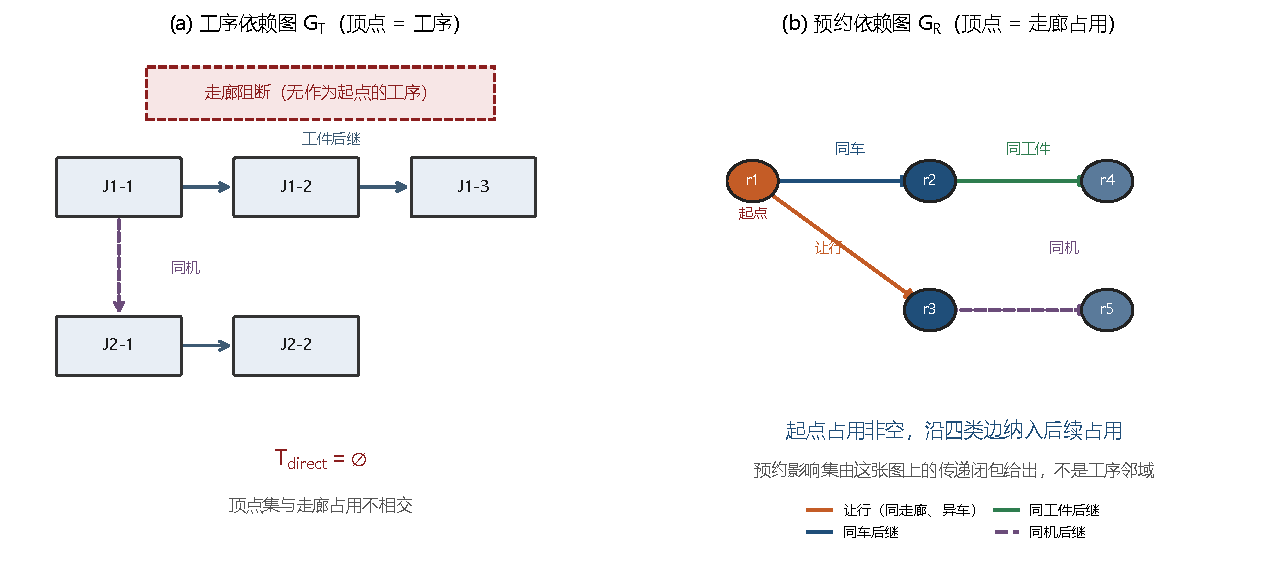
\includegraphics[width=\linewidth]{figures/fig_strc_graphs_CN}
\caption{两张图的顶点集不相交（构造示意）。
(a)~工序依赖图 \(G_T\)，顶点是工序，走廊阻断找不到作为起点的工序；
(b)~预约依赖图 \(G_R\)，顶点是走廊占用，从与阻断窗重叠的占用出发，沿四类依赖边
（让行、同车、同工件、同机；定义~\ref{def:dep}）纳入后续占用。}
\Description{并排两幅。左幅是工序依赖图，工件后继与同机后继连在工序方框之间，
顶部一条虚线框标出走廊阻断，阻断没有落在任何方框上。
右幅是预约依赖图，五个圆形顶点表示走廊占用，四条不同颜色的箭头分别标为
让行、同车、同工件与同机。}
\label{fig:graphs}
\end{figure}

\begin{table}[t]
\centering
\caption{本文常用记号}
\label{tab:notation}
\small
\begin{tabular}{@{}ll@{}}
\toprule
\textbf{符号} & \textbf{含义} \\
\midrule
\(G=(V,E)\), \(\tau_e\) & 走廊路网；走廊 \(e\) 的通行时间 \\
\(v_0\), \(\mathrm{loc}(m)\) & 装卸站；机械臂 \(m\) 所在节点 \\
\(x,\pi,y\) & 机器指派、加工顺序、车辆指派 \\
\(R\), \(r=(e,[t^s,t^e),k,u)\) & 预约表；一条半开占用（车辆 \(k\)，段标签 \(u\)）\\
\(G_T\) / \(G_R\) & 工序依赖图 / 预约依赖图 \\
\(\mathcal{S}^0,\mathcal{S}'\) & 扰动前排程、恢复后排程 \\
\(\mathcal{D},\,t_{\mathrm{now}}\) & 扰动事件、发生（决策）时刻 \\
\(T_{\mathrm{direct}},\,T_{\mathrm{impact}}\) & 工序依赖图上直接受扰的工序 / \(\theta\)-步纳入范围 \\
\(\mathrm{Src}(\mathcal{D})\), \(U\) & 作为起点的占用；允许改写的占用集合 \\
\(\mathrm{Cl}(\cdot)\) & 预约影响集（由 \STRC 得到）\\
\(\varphi\) & 受扰未来工序比例（规模扫描）\\
\bottomrule
\end{tabular}
\end{table}

\subsection{执行期假设}
\label{sec:assumptions}

执行期约定与物理设定如下。其中 A1--A4 由全部对照方法共用，以便把结果归因到重调度范围
如何划定，而不是模型差异；A5 只约束本文方法，全局重调度对照的允许动作更宽（见该条末句）：

\begin{enumerate}[label=\textbf{A\arabic*.},leftmargin=*,topsep=2pt,itemsep=2pt]
\item \textbf{初始排程可行。} \(\mathcal{S}^0\) 在扰动前通过无冲突校验；预约表与工序时间表一致。
\item \textbf{已完成占用不回溯。} 只改写 \(t^e>t_{\mathrm{now}}\) 的尚未结束占用
与未完工工序；\(t^e\le t_{\mathrm{now}}\) 的占用字段不可改写。
\item \textbf{单次、完全观测。} 扰动在 \(t_{\mathrm{now}}\) 被完整观测，且不与其它扰动叠加；
扰动流、预测误差与滚动响应不在本文范围内。
\item \textbf{走廊排他、缓冲充裕、车队同构单载。} 走廊仍为排他半开资源，阻断以附加占用
（或禁行窗）注入路由层。有限缓冲、充电、加减速与装卸时长不建模；
全部车辆在计划开始时空载停于 \(v_0\)。
\item \textbf{允许的恢复动作。} B 类扰动保持原机器指派 \(x\) 与加工顺序 \(\pi\)，只改路；
失败时扩大允许改写的占用集合。A 类故障额外允许：车辆故障把故障车从车队摘除并换车；
机械臂故障把未完工工序改派到其它可行机。加工顺序 \(\pi\) 始终不变，不重开搜索。
实验中的全局重调度对照可以改 \(x\) 与 \(\pi\)（第~\ref{sec:vs_r0}~节）。
\end{enumerate}

\subsection{扰动二分}
\label{sec:disturbance_classes}

\begin{definition}[A/B 类扰动]
\label{def:ab}
若扰动直接使某些工序的指派或\emph{可执行性}失效（机械臂故障、显著工时偏差、插单、
车辆故障等），称其为 \textbf{A 类}；若扰动只使某些走廊时窗不可用、而不使任何工序
不可执行（走廊阻断、走廊通行变慢等），称其为 \textbf{B 类}。
\end{definition}

\begin{remark}[车辆故障为何属于 A 类]
\label{rem:agv_class}
车辆故障不改动任何工序的机器指派，乍看应与走廊阻断同类。但定义~\ref{def:ab} 的判据是
\emph{可执行性}而非指派：车辆发生故障后，它承运的工序在原计划下无法开工，
故经「车辆\(\to\)所承运工序」的映射，工序依赖图上仍有作为起点的工序。这一归类把车辆故障
划到按工序划界能够给出非空范围的一侧。
只有当重调度方法维护了车--任务映射时，这些起点工序才非空；若方法只跟踪工序与机器
（AOR 的常见实现即如此），车辆故障同样会得到空范围。
第~\ref{sec:e6}~节按维护了该映射的口径报告 A 类结果。
\end{remark}

\begin{definition}[工序依赖图上的直接集与影响域]
\label{def:task_impact}
对扰动 \(\mathcal{D}\)，令 \(T_{\mathrm{direct}}(\mathcal{D})\) 为因机械臂故障、车辆故障或工序失效
而无法按原计划执行的工序集合。对 B 类走廊扰动约定 \(T_{\mathrm{direct}}=\varnothing\)。
在 \(G_T\) 上从 \(T_{\mathrm{direct}}\) 出发，按工件后继与同机后继纳入深度至多 \(\theta\) 的工序，
记为 \(T_{\mathrm{impact}}(\mathcal{D},\theta)\)。
\end{definition}

\begin{definition}[作为起点的占用]
\label{def:seeds}
起点集 \(\mathrm{Src}(\mathcal{D})\subseteq R\) 按扰动类型给出，一律只取
\(r.t^e>t_{\mathrm{now}}\) 的占用。
\begin{enumerate}[label=(\alph*),leftmargin=1.6em,itemsep=0.15em]
\item \textbf{走廊阻断/降速} \(\mathcal{D}=(e,[t_a,t_b))\):
\(\{\,r:\ r.e=e,\ [r.t^s,r.t^e)\cap[t_a,t_b)\neq\varnothing\,\}\)。
多处短暂阻断时取各窗起点占用之并。两者共用这条起点规则（原排程按时长未缩放的 \(\tau\) 写出，
与窗重叠的占用都已失效），故划定须改写的占用时二者给出同一个预约影响集——第~\ref{sec:e6}~节据此说明
为何不把二者的划界结果算作两次独立验证；改路时二者处理不同：阻断写为禁行窗，
降速只按倍率缩放与窗重叠部分的通行进度。
\item \textbf{车辆故障} \(\mathcal{D}=(k)\)：该车在 \(t_{\mathrm{now}}\) 之后的全部占用
\(\{\,r:\ r.k=k\,\}\)。
\item \textbf{机械臂故障} \(\mathcal{D}=(m,F)\),\(F\) 为该机上尚未完工的工序：
对每个工件取 \(F\) 中最小工序号 \(i_{\min}(j)\)，起点占用为各工件自该工序起（含）的全部
尚未结束占用。之所以沿工件链向后取而不只取该工序自身，是因为进站运输可能已在
\(t_{\mathrm{now}}\) 前结束，若只取自身，预约影响集会短于工序依赖图上的影响域，对照即不公平。
\end{enumerate}
\end{definition}

\begin{prop}[B 类上工序依赖图给出空范围]
\label{prop:miss}
设 \(\mathcal{D}\) 为走廊阻断。若采用定义~\ref{def:task_impact} 对 B 类的约定，则
\(T_{\mathrm{direct}}(\mathcal{D})=\varnothing\)，从而对任意有限 \(\theta\ge 0\) 有
\(T_{\mathrm{impact}}(\mathcal{D},\theta)=\varnothing\)。
若此外 \(\mathrm{Src}(\mathcal{D})\neq\varnothing\)，则 \(\mathcal{S}^0\) 在 \(\mathcal{D}\) 下不可行。
\end{prop}

\begin{proof}
走廊阻断只使走廊时窗不可用而不使任何工序不可执行，故按定义~\ref{def:ab} 属 B 类。
这一步用到两条前提：阻断窗 \([t_a,t_b)\) 有限，且由假设 A4 缓冲充裕，车辆可在窗外通行；
因而即使阻断期内路网被割断，也没有工序变得不可执行，只是被推迟。若阻断无限期、
或缓冲不足以支持等待，该扰动按定义~\ref{def:ab} 就该归 A 类，不在本命题范围内。
既属 B 类，
再由定义~\ref{def:task_impact} 对 B 类的约定，\(T_{\mathrm{direct}}=\varnothing\)。
\(\theta\)-步纳入的起点为空，故 \(T_{\mathrm{impact}}=\varnothing\)。
若存在 \(r\in\mathrm{Src}(\mathcal{D})\)，则 \(r\) 的占用区间与禁行窗相交。
将 \(\mathcal{D}\) 解释为该走廊上的强制占用后，\(r\) 与禁行窗在同一排他资源上时间重叠，
违背半开时窗无冲突条件（假设 A4 的走廊排他），故 \(\mathcal{S}^0\) 不可行。
\end{proof}

命题~\ref{prop:miss} 是问题层面上的反例。前半句由定义~\ref{def:task_impact} 对 B 类的约定直接得到
（工序依赖图按定义不含走廊占用之间的让行关系，因而无法刻画走廊阻断）；
非平凡的是后半句——起点占用非空时原排程已经不可行，
因而「工序依赖图上范围为空 \(\Rightarrow\) 无需重调度」在用时间窗预约走廊的设定下不成立。
该反例不依赖任何修复算法；实验第~\ref{sec:experiments}~节给出算例规模。

\subsection{恢复问题}
\label{sec:recovery_problem}

\begin{problem}[按预约表划定范围的有界修复]
\label{prob:recovery}
给定可行排程 \(\mathcal{S}^0\)、扰动 \(\mathcal{D}\) 与时刻 \(t_{\mathrm{now}}\)，
求 \(\mathcal{S}'\)，使得：
(i)~\(\mathcal{S}'\) 在 \(\mathcal{D}\) 下通过无冲突校验；
(ii)~未纳入改写范围的占用，其走廊、时段与车辆尽可能与 \(\mathcal{S}^0\) 一致；
(iii)~算法耗时受预算约束。
次级目标为完工时间 \(C_{\max}(\mathcal{S}')\)。
\end{problem}

求解拆为两步：先划定允许改写的占用集合 \(U\subseteq R\)；
再只对 \(U\) 内运输改路，集外占用保持原计划。
本文用 \(\mathrm{Cl}(\mathrm{Src})\) 给出 \(U\)；对照则用工序依赖图上的影响域诱导出预约子集。

%% =====================================================================
